% This file was created by tikzplotlib v0.9.8.
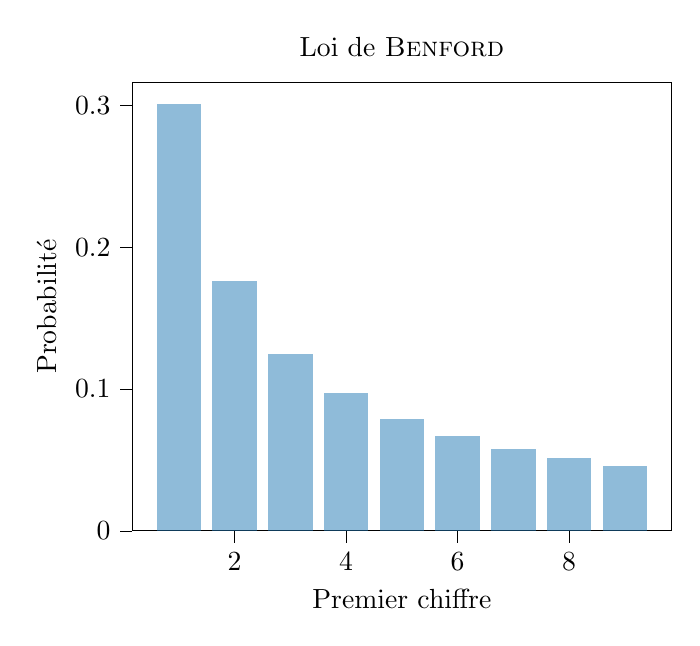
\begin{tikzpicture}

\definecolor{color0}{rgb}{0.12156862745098,0.466666666666667,0.705882352941177}

\begin{axis}[
tick align=outside,
tick pos=left,
title={Loi de \textsc{Benford}},
x grid style={white!69.0196078431373!black},
xlabel={Premier chiffre},
xmin=0.16, xmax=9.84,
xtick style={color=black},
y grid style={white!69.0196078431373!black},
ylabel={Probabilité},
ymin=0, ymax=0.31608149544718,
ytick style={color=black}
]
\draw[draw=none,fill=color0,fill opacity=0.5] (axis cs:0.6,0) rectangle (axis cs:1.4,0.301029995663981);
\draw[draw=none,fill=color0,fill opacity=0.5] (axis cs:1.6,0) rectangle (axis cs:2.4,0.176091259055681);
\draw[draw=none,fill=color0,fill opacity=0.5] (axis cs:2.6,0) rectangle (axis cs:3.4,0.1249387366083);
\draw[draw=none,fill=color0,fill opacity=0.5] (axis cs:3.6,0) rectangle (axis cs:4.4,0.0969100130080564);
\draw[draw=none,fill=color0,fill opacity=0.5] (axis cs:4.6,0) rectangle (axis cs:5.4,0.0791812460476248);
\draw[draw=none,fill=color0,fill opacity=0.5] (axis cs:5.6,0) rectangle (axis cs:6.4,0.0669467896306132);
\draw[draw=none,fill=color0,fill opacity=0.5] (axis cs:6.6,0) rectangle (axis cs:7.4,0.0579919469776867);
\draw[draw=none,fill=color0,fill opacity=0.5] (axis cs:7.6,0) rectangle (axis cs:8.4,0.0511525224473813);
\draw[draw=none,fill=color0,fill opacity=0.5] (axis cs:8.6,0) rectangle (axis cs:9.4,0.0457574905606751);
\end{axis}

\end{tikzpicture}
